% #############################################################################
% This is Chapter 2
% !TEX root = ../main.tex
% #############################################################################
% Change the Name of the Chapter i the following line
\fancychapter{Background}
\cleardoublepage
% The following line allows to ref this chapter
\label{chap:back}

	The development of an algorithmic-based framework for optimization, applicable to architectural domains, requires a careful review over the current literature on \ac{BPO} practices and limitations. 
	
	Firstly, the \textit{ad-hoc} nature of the functions used for performance assessment in \ac{BPO} motivates the application of a special class of optimization algorithms, the derivative-free algorithms. Within this class, different categories emerge, emphasizing the algorithms' different properties and search strategies. Applying the adequate algorithm to a certain problem may potentially increase the efficiency of an optimization process. 
	
	Secondly, there are multiple approaches to optimization that might be considered. Generally, \ac{BPO} practices include the simultaneous optimization of multiple aspects. However, they often opt for simpler specifications, often disregarding all but one of the initially considered aspects. 

	Finally, currently available architectural design optimization tools explore the parametric models produced in visual programming environments, such as Grasshopper and Dynamo. These visual programming environments are implemented as plug-ins, which are tightly integrated with \ac{CAD} and \ac{BIM} tools, respectively. As a result, the connection between optimization tools and visual design workflows becomes seamless and friendlier. Additionally, these optimization tools usually expose a \textit{ready-to-run} interface, which is very appealing to most \ac{BPO} practitioners~\cite{Cichocka2017SURVEY}.
	
	
	
% #############################################################################
\section{Derivative-Free Optimization}
\label{sec:dfo}

	Different optimization algorithms can solve, more or less efficiently, specific optimization problems, depending on their characteristics. Particularly, for optimization problems explicitly defined through mathematical formulations, algorithms that explore the information from the derivatives of such formulations to guide the search for optimal solutions are very efficient. These algorithms are referred to as classical gradient-based algorithms. However, when neither the mathematical form, nor the information about the derivatives is easily available, it becomes necessary to explore other classes of algorithms. Fortunately, derivative-free algorithms are remarkably suitable for addressing these problems, as they do not use information about the objective functions' derivatives to find optimal solutions, instead, they treat the objective functions as \textit{black-boxes} and guide the search based on the result of previously evaluated solutions~\cite{Rios2013}.
	
	In architecture, it is often impossible to attain a mathematical formulation for the objective functions, especially for complex designs. Alternatively, architects frequently use simulation tools as means to replace the closed-form mathematical expressions relating design's parameters to the objective functions~\cite{Wortmann2016BBO}. As a consequence, information about the objective functions becomes difficult to attain, often requiring excessive amounts of resources. This lack of information prompts the need for algorithms that treat these functions as \textit{black-boxes}. A simple approach is to systematically experiment with different parameter values until the best solutions are found, whereas a second, and more complex, approach is to use derivative-free optimization algorithms, also commonly referred to as black-box optimization algorithms within the architectural community~\cite{Wortmann2016BBO}. % Despite its simplicity, experimentation-based approaches, such as Monte Carlo Sampling and Latin Hypercube Sampling~\cite{Giunta2003DOE}, might not always be advisable, particularly when dealing with time-consuming functions as is the case of architecture. In such cases, derivative-free algorithms might be more appropriate, yielding better solutions in less time.

	Derivative-free algorithms allow to overcome the difficulty of deriving analytical forms that has has been rising with the increase of building design's complexity.~\cite{Machairas2014}. For this reason, derivative-free algorithms are sought as useful tools to optimize designs, having been applied extensively to optimize building designs' manifold aspects. Among the numerous studies that apply derivative-free optimization algorithms to optimize building designs, we refer to the distinct works of Wortmann~\cite{Wortmann2016BBO,Wortmann2015AdvSBO,Wortmann2017GABESTCHOICE,Wortmann2017Opossum}, Evins~\cite{Evins2011,Evins2012MOO,Evins2013}, and Waibel~\cite{Waibel2018} which cover the optimization of various aspects, including, among others, structural, lighting, thermal, energy consumption, and carbon-emissions. 
	
	For the past decades, the constant development and improvement of derivative-free optimization algorithms led to a diversified tools' gamut, each with its own characteristics and limitations. While the main ideas behind each algorithm's category seem to be more or less recognized throughout the architectural community, the lack of standards make it difficult to decide which definitions to convey~\cite{Rios2013, Wortmann2017ADO}. The currently most relevant classifications are: (1) the one presented by Rios et al.~\cite{Rios2013} that, based on the functions being used to guide the search process, classifies the algorithms into direct search or model-based algorithms; and (2) the classification provided by Wortmann et al.~\cite{Wortmann2017ADO}, which first subdivides the algorithms in two groups according to the number of solutions generated in each iteration, namely metaheuristics and iterative algorithms, and only then proceeds to classify iterative algorithms as direct search or model-based algorithms, depending on the function that is used during the search. 

	This thesis will consider an approach similar to the one proposed by Wortmann~\cite{Wortmann2017ADO} by exploring the concepts of metaheuristics, direct-search, and model-based algorithms. Albeit the apparent chasm between these classifications, some algorithms draw ideas from distinct classes, thus emphasizing not only the blurred lines of such categorizations, but also the difficulties that lie with the definition of more standardized classifications. 
	
	The following sections describe each class and its intrinsic characteristics, proceeded by a brief comparison among them in light of the architectural design practice. 	

% ----------- Subsection
\subsection{Direct Search Algorithms}
\label{ssec:direct-search}

	Although there seems to be no precise definition for direct search algorithms~\cite{Kolda2003}, these are often identified as algorithms that iteratively~\cite{Kolda2003,Wortmann2016BBO}: (1) evaluate a finite sequence of candidate solutions, proposed by a simple deterministic strategy; and (2) select the best solution obtained up to that time. They are sought as valuable tools to address complex optimization problems, not only because most of them were proved to rely on solid mathematical principles, but also due to their good performance at initial stages of the search process~\cite{Rios2013, Wortmann2016BBO}. 
	
	The main limitations of the algorithms in this class is their performance deterioration with the increase on the number of input variables, and their slow asymptotic convergence rates as they become closer to the optimal solution~\cite{Kolda2003}.

	Some examples of relevant direct-search algorithms include \ac{HJ}~\cite{Hooke1961}, \ac{NMS} method~\cite{Nelder1964}, SUBPLEX~\cite{Rowan1990}, \ac{DIRECT}~\cite{Jones1993DIRECT}, among others.
		
% ----------- Subsection
\subsection{Metaheuristics Algorithms}
\label{ssec:metaheuristics}

	In the original definition~\cite{Glover2003Metaheuristics}, these algorithms were solely based in the interaction between local improvement procedures, called heuristics, and higher-level strategies, called metaheuristics. On the one hand, heuristics are techniques that locate good solutions, but not necessarily the optimal, nor the correct solution, and that often consider the trade-off between precision and quality, and computational effort. On the other hand, a metaheuristic is an algorithmic framework that can be applied to different problems, with a few modifications to add problem-specific knowledge~\cite{Glover2003Metaheuristics}, if so is desired. Moreover, a metaheuristic is a higher-level strategy that extends the capabilities of heuristics by combining one or more heuristic methods (referred to as procedures), while being agnostic to each heuristic. The ```meta'' classification of these algorithms results from the fact that they control the heuristics applied in the process.

	Throughout time, this class has grown to include any algorithm that includes simple heuristics to locate good solutions in complex design spaces, while considering the trade-off between precision, quality, and computational effort of the solutions. These algorithms often rely on randomization, and biological or physical analogies, to perform robust searches and to escape local optima~\cite{Glover2003Metaheuristics, Wortmann2016BBO}. Additionally, their non-deterministic and inexact nature confers them the ability to effortlessly handle complex and irregular objective functions~\cite{Wortmann2017GABESTCHOICE}, as well as, to easily adapt to \ac{MOO} contexts, or even to provide domain-specific knowledge through the heuristics~\cite{Wortmann2017GABESTCHOICE}.
	
	Metaheuristics are efficient optimization algorithms when provided with sufficient amount of time to do the necessary objective function evaluations~\cite{Conn2009}. However, advantages can quickly become disadvantageous by simply changing the application context. This is the case of \ac{BPO} in the architectural practice, where each evaluation is a time-consuming task and the execution of thousands of evaluations rapidly becomes an infeasible scenario. Due to their stochastic nature, limiting the number of evaluations has severe repercussions, both on the convergence and performance guarantees~\cite{Hasancebi2009}. 
	
	In the architectural design context, some of the most relevant metaheuristics algorithms include the \ac{PSO} algorithms, some evolutionary algorithms, such as \ac{GA}, \acp{ES}, and even local search algorithms like tabu search and simulated annealing. We refer the interested reader to~\cite{BlumRoli2003Metaheuristics,Glover2003Metaheuristics} for more details about these metaheuristics algorithms.
	
% ----------- Subsection
\subsection{Model-based Algorithms}
\label{ssec:model-based}
	Model-based algorithms are effective handlers for time-consuming problems, where sensitive information is expensive to collect~\cite{Forrester2009SBO, Wortmann2016BBO}. These problems are characterized by the large time complexity associated with the computation of the values of the objective function, and by the absence of previous knowledge about the objective function. Model-based algorithms are able to provide instant estimates of a design’s performance, by supplementing or replacing the original objective function by its approximation~\cite{Wortmann2016BBO}. This approximation, called the surrogate, is generated from a set of known objective function values, and is then used to determine the promising candidate solutions to evaluate next. These candidate solutions are then used to improve the surrogate and this process is repeated until a stopping condition is satisfied~\cite{Koziel2011}.

	Despite having a well-defined analytical form, which makes computations on the surrogate model more efficient than on the original objective function, the surrogate is only an approximate representation of the original function, and, therefore, must be constantly updated to guarantee a reasonable locally accurate representation~\cite{Koziel2011}. \Cref{fig:sbosexample} illustrates a surrogate that is accurate near the initial solutions. However, as we analyse solutions far from the initial ones, the accuracy of the surrogate model worsens.
	
	% Begin Figure: SBO Simple Example ----------------------------
	\begin{figure}
	\centering
	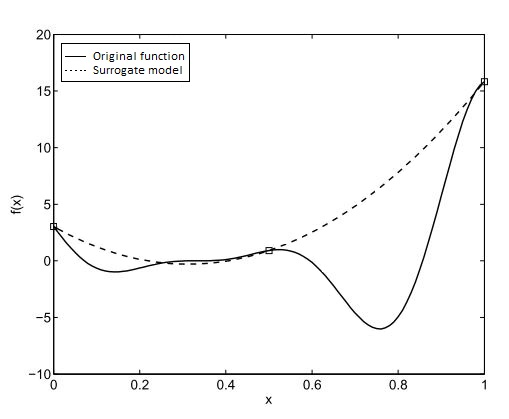
\includegraphics[width=8cm]{Images/Background/sbosexample.JPG}
	\caption[Example of a surrogate model]{Original function and corresponding surrogate model, created based on three initial solutions (squares). This image was retrieved from~\cite{Koziel2011}.}
	\label{fig:sbosexample}
	\end{figure}
	% End Figure -------------------------------------------------------
	
	Nowadays, the existing plethora of techniques applicable to the generation of surrogate models range from trust region methods to \ac{ML} techniques. These techniques can be used to create (1) local surrogates, i.e., models where the approximation to the objective function is built around a certain point, and (2) global surrogates, i.e, models where the approximation is generated from all the obtained points. Whilst the former relies on the construction of simple, partial models of the objective function, the latter relies on the creation of a full model. The creation of the full model, requires balancing the need for improving the accuracy of the model by exploring broader regions in the solution space, with the need for improving the value of the objective function by exploiting promising regions~\cite{Koziel2011}. This balance is determined by a strategy that selects the next promising solution to evaluate.
	
	Undoubtedly, the best feature of model-based algorithms is the reduction in the total optimization time. This is particularly relevant in the context of \ac{BPO}, where each simulation may take seconds, minutes, hours, days, or even weeks to complete. However, the lower availability and the lack of necessary technical knowledge to implement or incorporate these algorithms into optimization processes are still obstacles to a broader adoption of this approach. Notwithstanding the existence of different studies involving \ac{ML} techniques for the creation of full surrogate models~\cite{Koziel2011, Forrester2009SBO}, such as \acp{NN}, \acp{SVM}, \acp{RBF}, and \acp{RF}, among others, only a few have actually been applied in the context of architecture. This scenario is even more self-evident when we shift from the single- to multi-objective optimization context.

% ----------- 
\subsection{Comparison}
\label{ssec:comparison}

This section considers the applicability of different classes of derivative-free optimization algorithms for architectural design. The multidisciplinary aspect of building design raises distinct problems, ranging from well-behaved problems with simple, unimodal, convex functions to more ill-behaved problems with irregular, multimodal objective functions~\cite{Wortmann2017ADO}. In addition to problem's diversity, the time complexity associated to function evaluations also becomes an important factor to consider, when pondering each category's impact on \ac{BPO} problems.

The problems' plethora within performance-based design is vast: a specific optimization algorithm may perform well for some problems and have a terrible performance in other problems~\cite{Wortmann2017GABESTCHOICE, Fang2017}. This idea resembles the ones captured in Wolpert's \acp{NFLT} for optimization, which state that any algorithm's worse performance over some classes of problems offsets its better performance in other classes. Because of the distinct nature of architectural design problems, the arguments applied in architecture are not necessarily applicable to the other fields, like science and engineering. 
	
Inevitably, the same building design description might yield different problem descriptions according to the performance aspects being considered. Some algorithms might explore certain descriptions more effectively than others, e.g., because the objective functions describing the lighting and structural behavior of a certain design may have completely different properties. In an attempt to exploit this property, \ac{BPO} practitioners often dedicate a small amount of their total time budget to test various algorithms and different setup parameters, before finally settling for an optimization algorithm~\cite{Hamdy2016}.	
	
Regarding the different algorithms' categories, it is interesting to see the metaheuristics' popularity among researchers and practitioners. The main reasons behind the idolization of the metaheuristics are their (1) inherent simplicity, (2) ease of implementation, and (3) wide applicability to different domains~\cite{Wortmann2017ADO}. Unfortunately, other categories do not benefit from such properties, which is a limitation towards their application in architectural domains. Moreover, the lack of easy-to-use tools involving algorithms from other categories are also limiting their application in architectural contexts. Firstly, the existing non-metaheuristic tools are usually available as programming libraries, instead of being integrated in architectural design workflows. As a result, to use the optimization algorithms, architects often need some programming knowledge to create the scripts to integrate the algorithms into the design workflow. However, since architects typically lack the required knowledge, they tend to struggle with the scripts' production and, eventually, opt for using friendlier metaheuristics ready-to-use tools. Given this facts, it is not surprising that most of the existing building design optimization literature ends up focusing on the application of algorithms from the metaheuristics category~\cite{Hamdy2016,Nguyen2014,Evins2013}. 
		
However, in the light of the \acp{NFLT}, the need for more short-term efficient optimization approaches fostered the development of tools exposing algorithms with different properties. Particularly, plug-ins like Goat~\cite{GOAT} and Opossum~\cite{Wortmann2017Opossum} enable the usage of algorithms from both direct search and model-based classes. These tools expose optimization algorithms from the NLopt~\cite{NLOPT} and RBFOpt~\cite{RBFOPT} frameworks, respectively, providing friendly, ready-to-use interfaces within Grasshopper~\cite{GRASSHOPPER}, a visual programming environment that enables the parametric design and performance evaluation of building designs for different values of the parameters. For the past few years, few works have compared different algorithms using these tools with the ones available in other metaheuristics tools (e.g., Galapagos~\cite{GALAPAGOS}, Octopus\cite{OCTOPUS}, Optimo~\cite{OPTIMO}, Silvereye~\cite{Cichocka2017SILVEREYE}).
	
Although the results may vary, in general, direct search and surrogate-based algorithms seem to be more effective than the metaheuristics ones in initial stages of the optimization process~\cite{Wortmann2017,Wortmann2016BBO,Wortmann2017GABESTCHOICE}. Even some metaheuristics algorithms can be very effective approaches for some optimization problems~\cite{Waibel2018}. One can explore these performance fluctuations to find the most effective optimization algorithm for a specific problem. This performance gain can be determining in the overall optimization time, especially when complex and time-consuming simulations are involved. Indeed, several authors ~\cite{Wortmann2016BBO,Hamdy2016} suggest that the selection of the optimization algorithm should be based on the results of several tests with different methods for a fixed number of evaluations or a fixed amount of time. 

Optimization is a useful tool to address both single and multi-objective problems. In architecture, most optimization applications focus on single-objective problems and cover the three different derivative-free algorithms classes. However, the same does not happen with multi-objective problems, with only one of the classes being extensively applied to \ac{MOO} building design: the metaheuristics~\cite{Hamdy2016}. The main reason behind metaheuristics popularity is their broader adaptability to both varying degrees of complexity and to different problem domains~\cite{BlumRoli2003Metaheuristics}.
	
Recent developments in multiple surrogate-assisted \acp{MOEA} in the fields of science and engineering~\cite{Zapotecas-Martinez2016,Hussein2016} made it possible to decrease the number of expensive evaluations in \ac{MOO} problems. Generally, these techniques combine metaheuristics methods, which find more than one solution within a single execution, with surrogate models, which are approximations of the original objective functions. Diaz-Manriquez et al.~\cite{Diaz-Manriquez2016} provide a comprehensive overview of surrogate-assisted techniques for \ac{MOO} from the engineering perspective. 

The following sections focus on the current \ac{BPO} practices both for \ac{SOO} and \ac{MOO}, the currently available tools, and the advantages and disadvantages of each approach.
	
% #############################################################################
\section{Single-Objective Optimization}
	
\ac{SOO} processes aim to find the best solution with respect to a unique objective function. This function is described in terms of the values of the problem's parameters. \Cref{eq:soo} illustrates an example of a mathematical unconstrained minimization \ac{SOO} problem, where $f$ represents the single objective function and $x$ represents the vector of parameters.
		
\begin{equation} \label{eq:soo}
   	\min f(x) 
\end{equation}

Generally, the computational complexity of optimization processes is exponential on the number of objectives and, consequently, the more objectives, the more expensive these processes are. In particular, \ac{SOO} processes rely exclusively on a single objective function and, therefore, are usually less time-consuming than the \ac{MOO} processes. The gains in computational resources become particularly relevant when considering simulation-based objective functions. For instance, in the case of building design, most problems include simulation-based objective functions. As a result, architects commonly opt for \ac{SOO} processes: either by simply considering a single objective, or, in the case of problems involving multiple conflicting objectives, by combining them in a unique function as it will be further explained in \cref{subsec:preferencesarticulation}.
	
A literature review over the architectural practice will evidence the prevalence of \ac{SOO} algorithms. Firstly, single-objective problems are easier to model. Secondly, plug-ins, like Galapagos and Goat, allow to easily address single objective building design problems, hence enabling to solve simpler optimization problems and reducing the total complexity of optimization processes. Finally, these plug-ins expose different derivative-free optimization algorithms, enabling the selection of the best algorithm to specific problems and potentially improving the optimization processes' complexity~\cite{Wortmann2016BBO}. 
			
Despite its lower optimization time, these processes are also usually less informative than the ones for multi-objective problems. Particularly, in the architectural practice, building design often involves different conflicting aspects, such as thermal, energy consumption, lighting, among others. In such situations, one is interested in obtaining a view over the compromises between conflicting aspects in order to make an informed decision.
	
% #############################################################################
\section{Multi-Objective Optimization}

\ac{MOO} belongs to the set of problems concerned with the optimization of more than one objective simultaneously. The addition of other, potentially conflicting, objectives to the optimization process requires the re-definition of \textit{optimality}. 

While in \ac{SOO} problems we expect the optimal solution to be the set of parameters that achieve the best\footnote{For simplification purposes, we simply refer to the optimal solution as being the best. When dealing with a minimization problem, the best solution is the one that achieves the lowest value of the objective function, whereas in maximization problems, the best solution is the one achieving the highest value of the objective function.} objective value possible, in multi-objective the best possible configuration for one of the objectives is rarely the best possible configuration for all other objectives as well, which results from the fact that these objectives are often contradictory. In order to be able to compare different multi-objective solutions, these problems are often addressed considering the Pareto optimality (or Pareto efficiency) concept. This concept, named after the economist Vilfredo Pareto, defines an optimal solution as being a solution for which it is impossible to improve an objective value without deteriorating others. Such a solution is also said to be non-dominated or noninferior, and the set of non-dominated solutions is called the Pareto Front. An example of a two-objective minimization problem is illustrated in Figure~\ref{fig:paretofrontier}. The two objectives are $f_1$ and $f_2$ and the solutions shown in orange are non-dominated. The goal of optimization algorithms is to find, in the search space, design solutions that lie on the Pareto Front.

% Begin Pareto-Optimization Figure -------------------------------------------------------
\begin{figure}
\centering
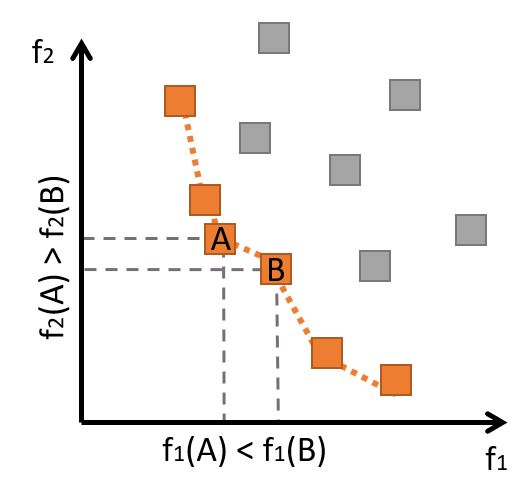
\includegraphics[width=5cm]{Images/Background/pareto-front.JPG}
\caption[Example of a bi-objective optimization problem]{Representation of the set of non-dominated (orange squares) and dominated (gray squares) solutions for a two-objective minimization problem. The Pareto front is composed of all the non-dominated solutions.}
\label{fig:paretofrontier}
\end{figure}
% End Figure -------------------------------------------------------

Building design is a complex task that frequently involves dealing with multiple conflicting objectives, such as maximum lighting comfort \textit{versus} maximum thermal comfort, or minimum energy consumption \textit{versus} maximum thermal comfort. The architect might follow different approaches depending on his knowledge and on his level of expertise. The following three sections describe the benefits and limitations of each approach. 

% ----------- 
\subsection{Design of Experiments}

The experimental or design of experiments approach is widely used in research and in practice to address both single and multi-objective problems~\cite{Fang2017}. Besides being intuitive and flexible, it can achieve a potentially better solution without having to deal with complex optimization algorithms. This approach evaluates designs generated with different combinations of design parameters. These combinations can be obtained through sampling methods, such as Full-factorial, Monte Carlo Sampling, and Latin Hypercube Sampling~\cite{Giunta2003DOE}, which generate different combinations of design to be evaluated. This approach returns multiple design solutions instead of just one, leaving the final choice in the hands of the architect.

Unfortunately, this approach does not guarantee that good solutions will be found. In fact, in most cases, new solutions are generated without taking advantage of the information obtained from previously evaluated designs. Consequently, the old information is not used to guide the search towards the most efficient designs and useless candidate designs can sometimes be evaluated. 

On the other hand, given its simplicity and flexibility, this approach allows architects to easily combine different processes in order to direct the search towards better design solutions. For example, the architect can choose a sampling method to generate different design variations, which are then evaluated. After analyzing the results of the evaluations, the architect may wish to explore regions of the design space near the most promising design solutions. In that case, he might constrain the design variations to lie within the promising regions, by updating the problem’s definition. The redefined problem is then subsequently sampled and redefined until the architect is satisfied with the quality of the obtained solutions.
	
Despite the constant need for manual intervention, the previous technique can be adapted to automatically extract information about the design problem itself, for example, to study the impact of design parameters in the performance. This process, commonly known as \textit{sensitivity analysis}~\cite{Saltelli2007}, has already been applied in the context of building design optimization~\cite{Tian2013}, not only to achieve better solutions, but also to enhance the performance of existing optimization algorithms, e.g., by dropping irrelevant parameters.

Overall, while it does not provide guarantees about the solutions’ optimality, this approach is simple, easy to use, and it is available in numerous tools. Moreover, although this process is not intelligent \textit{per si}, since the decisions are always made by the architect, it enables a more intelligent and informed design process, as it presents all the design variations generated and their associated performance.
	
% #############################################################################
\subsection{\textit{A Priori} Articulation of Preferences}
\label{subsec:preferencesarticulation}
This approach allows combining multiple objectives according to one’s preferences, using what is called a utility function \cite{Marler2004}, i.e., a function which ranks alternatives according to their utility for global performance. Among all the possible utility functions, the most commonly used is the weighted sum or linear scalarization \cite{Wortmann2017Opossum}. This function reduces multi-objective problems to single-objective ones by defining the objective function as the weighted sum of multiple objectives. The weights represent the relative importance of each objective to the architect and must be
defined before the optimization. The final objective function is then provided to a \ac{SOO} algorithm, which tries to find an optimal (or a near optimal) solution. \Cref{eq:scalarization} represents an unconstrained example of the mathematical definition of such approach, where $w_i$ is the weight associated to the objective $f_i$, and $n$ is the total number of objectives of the problem. 

\begin{equation} \label{eq:scalarization}
   	\min_{x \in X} \sum_{i=1}^n w_i f_i(x)
\end{equation}

One important consideration to have when following this approach is its sensitivity to the chosen weights, as different weights can yield potentially distinct results. Architects often use their experience or knowledge about the problem itself to set these weights properly, thus ensuring they obtain an optimal (or near optimal) solution.

Virtues of this approach, in architecture, include the ease of use, the availability, the heterogeneity of ready-to-use \ac{SOO} tools (e.g., Opossum, Goat, Galapagos, Silvereye), and the time required. %when compared to other \ac{MOO} approaches. % In general, because this preference-based approach focus in the retrieval of a single optimal solution that satisfies the previously defined preferences, it becomes more effective and less time consuming than other \ac{MOO} approaches, that either lack a more guided search or that aim at finding solutions that are optimal under different preference articulations. 

Overall, this approach enables a more intelligent design process because the algorithm uses knowledge about previously evaluated solutions to guide the search towards optimal regions of the design space. However, since the algorithms used are usually autonomous, architects are often removed from the optimization loop, thus losing control over the design optimization process. Moreover, most of these algorithms retrieve a single optimum and provide no other design options. This is a major drawback~\cite{Cichocka2017SURVEY}, as the architect either complies to the retrieved solution or he must rerun the optimization with another articulation of preferences. Either way, this optimization approach no longer provides enough information to make informed decisions.

% #############################################################################
\subsection{Pareto-based Optimization}

A more informative approach consists in the retrieval of a diverse and potentially heterogeneous set of Pareto-optimal solutions. When confronted with this set of optimal solutions, architects can compare different design options, according to different performance criteria, and make informed decisions about the compromises taken. \Cref{eq:pareto-based} is an example of a mathematical unconstrained minimization Pareto-based \ac{MOO} problem, where $F(x)$ represents the vector of $k$ objectives, and $f_i$ represent the objective function $i$.
		
\begin{equation} \label{eq:pareto-based}
   	\min \left\lbrace F(x) = \left[f_1(x), f_2(x), ..., f_k(x)\right] \right\rbrace
\end{equation}
    
On the other hand, in this approach, (1) the number of function evaluations is larger due to the need to find a set of optimal solutions instead of focusing on a single one, (2) the visual representation of the solutions’ objective space becomes problematic when the number of objectives is greater than three, and (3) the way the optimization problem is modeled has a direct impact on the quality of the solutions.

Notwithstanding the considerations above, a few studies concerning Pareto-based optimization emerged in the past years, evidencing its utility~\cite{Evins2013,Hamdy2016}. Moreover, recent works show that even though
approaches based on the \textit{a priori} definition of preferences are less time-consuming, they are not as desirable as Pareto-based approaches, as they return a single solution instead of multiple alternative solutions~\cite{Attia2013,Hamdy2016,Cichocka2017SURVEY}. In fact, Pareto-based approaches support the decision making process, providing a clear trade-off between the different objectives involved. Moreover, these multiple compromises represent different articulation of preferences from which the architect selects one. This approach is also called \textit{a posteriori} articulation of preferences.

Despite the growing trend of Pareto optimization approaches~\cite{Evins2013, Hamdy2016}, the lack of relevant benchmarks comparing the performance of different \acp{MOOA} in architecture is evident. 

% #############################################################################
\section{Quantitative Performance Indicators}

Despite the large interest in \ac{MOO}, the question of how to quantitatively compare the performance of different algorithms still remains unanswered. Firstly, in multi-objective problems, the number of objectives in the objective space is greater than the number of objectives in single-objective problems: the former considers a collection of vectors representing the Pareto-optimal solutions, whereas the latter considers real numbers. Secondly, it is often the case that the application of exact methods to \ac{MOO} contexts is impracticable due to the complexity introduced by underlying applications (e.g., simulation tools, physical experiments). In these cases, the generation of the true Pareto-optimal set is often infeasible, requiring vast computational resources to be generated. Thirdly, despite the availability of alternatives to exact methods, such as metaheuristics algorithms (e.g., evolutionary algorithms, particle swarm), these are not guaranteed to identify optimal trade-offs, instead yielding good approximations~\cite{Zitzler2003Metrics}. Finally, we are interested in knowing which of the non-exact algorithms yields better approximations for a given problem, hence prompting the need for assessing the performance of \acp{MOOA}.

The notion of performance includes not only the quality of the results, but also of the computational resources needed to generate such results. While the latter aspect is usually identical for both \ac{SOO} and \ac{MOO}, which either typically consider the number of expensive evaluations or the overall run-time on a particular computer, the quality aspect is considerably different. Because \acp{SOO} consider real-valued objective spaces, the quality is defined in terms of the objective function: the smaller (or larger) the value, the better the solution. However, \acp{MOO} consider vector-valued objective spaces, thus requiring another concepts like Pareto dominance. Unfortunately, when considering the Pareto dominance concept a few issues may arise, namely the possibility of two solutions being incomparable, i.e., when neither dominates the other, or having solutions in one set that either dominate or are incomparable to those in the other set of solutions and vice versa. 

Literature review evidences the existing struggle to define the meaning of quality with respect to approximation of Pareto-optimal sets~\cite{Knowles2002Metrics,Riquelme2015}. However, the quality of Pareto sets is usually evaluated in terms of three aspects: (1) cardinality, meaning larger sets of solutions, (2) diversity, meaning that solutions should be as uniformly distributed as possible, so as to obtain a representative set of solutions covering to larger extents the different trade-offs, and (3) accuracy, meaning that solutions should be as close as possible to the true Pareto-optimal set or Pareto Front. 

For the past decades, several indicators have been proposed to measure the quality of Pareto sets, ranging from unary quality measures, which assign each approximation set a number that reflects a certain quality aspect, to binary quality measures, which assign numbers to pairs of approximation sets, among others. This thesis considers a small but representative set of quantitative indicators to measure the quality of \acp{MOOA}' results with respect to the three aspects: cardinality, diversity, and accuracy. 

Literature review reveals the existence of dozens of indicators that consider either one of the mentioned aspects or a combination of them. In the following definitions we use the term \textit{approximation set} to denote the Pareto Front returned by the optimization algorithm, and we use the term \textit{reference set} to denote the true Pareto Front or, whenever that is not possible, an estimate of the true Pareto front. 
In this section, we list some of the most used indicators for assessing the performance of evolutionary \acp{MOO}~\cite{Riquelme2015}. 

\todo{Should I discuss disadvantages of these indicators?}

\subsection{Unary Indicators}
% ---------------------------
% Unary Indicators 
% ---------------------------
%% https://github.com/PastelBelem8/MscThesis/blob/metrics/src/indicators/MOOIndicators.jl
% Cardinality 
With regards to the cardinality aspect, there are essentially two indicators:
\begin{itemize}
\item \textbf{\ac{ONVG}} computes the number of non-dominated solutions in the approximation set.
\item \textbf{\ac{ONVGR}} computes the ratio of non-dominated solutions in the approximation set with regards to a reference set.
\end{itemize}

% || Diversity / Distribution ||
Conversely, there are more indicators that measure the distribution of solutions in the objective space, i.e., the diversity aspect of the approximation set:
\begin{itemize}
\item  \textbf{Spacing} (or Set Spacing) computes the variance of the Manhattan distances between each non-dominated solution and its closest neighbor. It measures how well-spaced the solutions from the approximation set are. A value of zero represents equally spaced non-dominated solutions. 
\item \textbf{Delta Indicator} (spread or $\Delta$) is similar to Spacing. However it calculates the normalized variance and uses the Euclidean distance instead.
\item \textbf{Maximum Spread} (or \textbf{$M_3^\ast$}) computes the Euclidean distance between the bounds of each objective dimension. It measures the extent of the objective space in each dimension by calculating the distance between the maximum and minimum of each objective. A greater value indicates larger coverage of the objective space.
\item \textbf{Entropy} uses the Shannon's entropy concept to measure the uniformity of the approximation set distribution. This indicator makes the assumption that each solution provides some information about its vicinities, thus modeling each solution with Gaussian distributions. These distributions add up to form a density function capable of identifying peaks and valleys in the objective space, corresponding to dense and sparse zones, respectively. 
\item \textbf{Diversity Metric} is similar to the Entropy indicator. However it projects the solutions of both the approximation set and the reference set to an hyperplane which is then subdivided uniformly. Then it computes the ratio between the number of intervals that have at least one non-dominated solution from both sets and the number of intervals that have at least one non-dominated solution of the reference set. Higher values of the diversity metric imply a better distribution and higher diversity of the approximation set when compared to the reference set itself. 
\end{itemize}

% || Accuracy ||
In terms of accuracy, the following indicators are frequently used to measure the convergence of the approximation set:
\begin{itemize}
% ER
\item \textbf{\ac{ER}} computes the proportion of false-positives in the approximation set, i.e., the ratio of optimal solutions in the approximation set that are not optimal in a given reference set. Lower values of \ac{ER}, represent better the approximated sets. 
% MPFE
\item \textbf{\ac{MPFE}} computes, for each solution in the approximated set, the minimum Euclidean distance to the closest solution in a given reference set, returning the maximum of those distances. In other words, it returns the maximum error of the approximated Pareto Front. Lower values of \ac{MPFE} imply better approximation sets. 
% Generational Distance
\item \textbf{\ac{GD}} computes the average distance of an approximation set to a given reference set by computing the average distance of the solutions in the approximation set to the nearest points in a given reference set. A value of $0$ indicates that all the solutions in the approximation set are in the reference set. This metric has also been called \textbf{$M_1^\ast$} in other works~\cite{Zitzler2000m1m3}.
\end{itemize}

Finally, there are also some indicators that provide insights about both the distribution of the solutions of the approximation set and its accuracy:
\begin{itemize}
% Hypervolume
\item \textbf{\ac{HV}} (or Lebesgue measure or S-metric) measures the size of the objective space covered by an approximation set, i.e., it measures the volume of the dominated space. It provides the unique and desirable properties of (i) Pareto \textit{compliance}, i.e., an approximation set which completely dominates another, will necessarily have a greater volume than the latter, and (ii) convergence guarantees, i.e., any approximation set that achieves the maximum possible volume is guaranteed to contain all Pareto-optimal solutions.
% Inverted GD
\item \textbf{\ac{IGD}} is the opposite of \ac{GD}, instead computing the average distance between a given reference set and the approximation set. \ac{IGD} computes the distance between each solution in the reference set and its closest solution in the approximation front, averaged over the size of the reference set. Smaller values of \ac{IGD} suggest better approximation sets, given that the reference set is well distributed.  \ac{IGD} is identical to a previous metric, known as \textbf{$D1_R$}. 
\end{itemize}


\subsection{Binary Indicators}

In situations where the original Pareto-optimal set is not available, the binary indicators provide a way to compare approximation sets with respect to all the aspects. Among the most used indicators, there are:
\begin{itemize}
\item \textbf{Two set coverage} (or C-metric) yields the number of solutions in one approximation set that are dominated by at least one of the solutions of the other approximation set. A value of $1$ suggests that the second approximation set is completely dominated by some solutions in the first one, whereas a value of $0$ represents the situation when none of the solutions of the second approximation set is covered by the first approximation set.
\item \textbf{Epsilon Indicators} ($\epsilon$) that gives a factor by which an approximation set is worse than another considering all objectives, i.e., given two approximation sets $A$ and $B$, it computes the smallest amount $\epsilon$ by which $A$ must be translated, so that every solution in $B$ is dominated by at least one solution in A. 
\item \textbf{R-metrics} consider a family of indicators where the quality of each approximation set is defined according to a set of utility functions, and the larger the utility value of some set, the better the quality. R-metrics declare that the best approximation set will be the one that is better with regards to most utility functions:
	\begin{itemize}
	\item \textbf{$R1$} determines whether the an approximation set is better, equal, or worse than the other. 
	\item \textbf{$R2$} computes the expected mean difference in the utilities of both approximation sets.
	\item \textbf{$R3$} computes the expected mean relative difference in the utilities of both approximation sets.
	\end{itemize}
\end{itemize}

% #############################################################################
\section{Optimization Tools in Architecture}
	
For years, multiple optimization frameworks have been developed. However, in order to be used within architectural practices, architects had to code the integration scripts to connect the simulation models for different variations of the parametric models and the optimization frameworks~\cite{Attia2013}. Moreover, these frameworks often lacked post-processing and visual features, which antagonized the readability and comprehension of the results~\cite{Attia2013,Nguyen2014}.
	
Several plug-ins have been developed in an attempt to reduce the limitations associated to the coupling of simulation tools and mathematical optimization frameworks, thus providing a seamless connection between the parametric models produced in computational design tools, like \ac{CAD} and \ac{BIM} tools, the simulation or analytical models, and the optimization frameworks. Given the visual nature of architects, these plug-ins provide friendly, ready-to-use optimization interfaces, which are usually coupled with a few post-processing and visual features to enhance the intelligibility of optimization results. 
	
Currently, existing optimization plug-ins are implemented on top of the visual parametric tools: Grasshopper~\cite{GRASSHOPPER} and Dynamo~\cite{DYNAMOBIM}. In \Cref{fig:opt-plugins}, we represent the most relevant optimization plug-ins among \ac{BPO} practitioners: Galapagos, Goat, Octopus, Opossum, and Silvereye implemented on top of Grasshopper, and Optimo implemented on top of Dynamo. In the following sections we briefly discuss each plug-in.
	
% Begin Optimization Plug-ins Figure -------------------------------------------------------
\begin{figure}
\centering
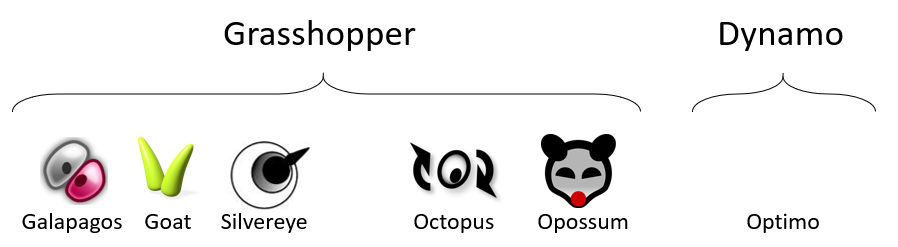
\includegraphics[width=\textwidth]{Images/Background/opt-plugins.PNG}
\caption[Optimization Frameworks in the Architectural Practice]{Optimization frameworks currently used in architectural practices.}
\label{fig:opt-plugins}
\end{figure}
% End Figure -------------------------------------------------------

\subsection{Galapagos}
\label{subsec:galapagos}
% General description of Galapagos, intuition
Galapagos is a well-known metaheuristic-based optimization plug-in developed for designers and implemented on top of Grasshopper. David Rutten developed Galapagos, a generic platform designed to allow the application of metaheuristics algorithms by non-programmers to solve a wide variety of problems. Moreover, to enable its usage by non-experts, the optimization solver assumes default values for the different available algorithms. 

% Available Algorithms
Galapagos provides two metaheuristics algorithms, namely, the genetic algorithm, inspired by biological evolution processes, and the simulated annealing, motivated by the metallurgical process of annealing \cite{Brownlee2011}. Although both algorithms are the basis for a large variety of extensions and/or specializations, supporting different heuristics, we will not provide a full description of such extensions, instead referring the interested reader to proper literature throughout this section. 

% Algorithms description
As evolutionary algorithms, genetic algorithms explore Darwinian natural selection concepts, such as heredity, reproduction, and natural selection, and genetics concepts and mechanisms, including genes, chromosomes, recombination, crossover, and mutation, in order to search for better solutions in the solution space. More concretely, genetic algorithms generate an initial random set of solutions, called population, which is then iteratively evolved, creating new generations. The evolution process is comprised of four main phases: (1) adaptability, where individuals of the population are assigned a suitability or fitness value; (2) selection, where pairs of individuals are selected for reproduction, based on a probabilistic function which is proportional to each individual's fitness value; (3) crossover, where the genotypes of the selected individuals are recombined to produce new individuals; and (4) mutation, where new individuals are subjected to random copying errors with a certain probability. While earlier generations are usually diverse, final generations are often very similar to the fittest individuals, i.e., we observe an intensification of the traits of the most suitable individuals, thus emulating the mechanism of natural selection, described by Darwin \cite{Brownlee2011}. Besides genetic algorithms \cite{Golberg1989,Holland1992}, evolutionary algorithms encompass other algorithms such as Genetic Programming~\cite{Koza1992}, Evolution Strategies \cite{Schwefel1981}, Differential Evolution \cite{Storn1997}, among others. 
	
Besides genetic algorithms, Galapagos also provides a metaheuristics global optimization physical algorithm, the simulated annealing. Resemblant of hill climbing algorithms, where new candidate solutions are randomly sampled, this algorithm iteratively re-samples the solution space aiming at finding an optimal solution. During the search, the algorithm is propitious to accept the re-sampled solutions with lower performance, according to a probabilistic function that becomes more discerning of the quality of the samples over the execution of the algorithm, thus resembling the natural annealing process~\cite{Brownlee2011}. 

% Usability, how to use it
To use one of Galapagos' optimization solvers, architects must define a Grasshopper's script in three parts: (1) Input, where they specify the design's parameters; (2) Generation, where they create the design's algorithmic model that when instantiated with the parameters' values will generate the 3D model; and (3) Analysis, where they define the analysis function or objective function which they ought to optimize. To that end, architects use Grasshopper's components, such as \textit{Sliders}, values lists, area, distance, and other analytical-like components to define the programs. In order to use Galapagos, optimization variables must be defined in terms of \textit{Sliders}, which enable the specification of numerical ranges with both lower and upper bounds, whereas the value of the objective function must be a \textit{Number} (\textit{Num}) component. Both the \textit{Sliders} and the \textit{Num} components connect to the input entry and to the output entry of the Galapagos' component, respectively, i.e., the genome and the fitness entries. 

% Begin Galapagos-Options Figure -------------------------------------------------------
\begin{figure}
\centering
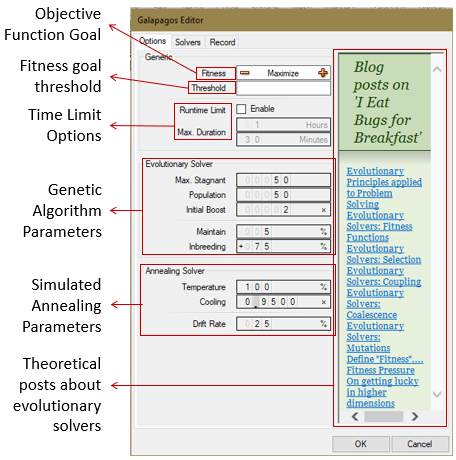
\includegraphics[width=0.5\textwidth]{Images/Background/Galapagos/galapagos-options-menu.PNG}
\caption[Galapagos algorithm's configuration menu]{Galapagos Options menu for parametrizing the solvers}
\label{fig:galapagossetup}
\end{figure}
% End Figure -------------------------------------------------------	

% Graphical interface, benefits of interface
After defining the problem, the architect double clicks the Galapagos component and is presented with its \ac{GUI} (see \Cref{fig:galapagossetup}). This interface is friendlier, simpler, and easier to use than other approaches, requiring no integration efforts, nor any programming or algorithm's knowledge in order to setup and use it. For all these reasons, Galapagos is particularly popular amongst architects~\cite{Wortmann2017ADO}, not only satisfying the visual nature of architects, but also supporting graphical views that yield feedback about the course of the optimization process. 

% Graphical interface
Particularly, Galapagos supports four graphical views for the genetic algorithm (see \Cref{fig:galapagosvisualmenu}-left), namely (1) the fitness graph, representing the distribution of fitness values in the population per generation, (2) the similarity representation graph, where genetically similar solutions are closer to each other and where solutions contributing to the next offspring and solutions that do not contribute are represented with a black dot and a red cross, respectively, (3) the parallel coordinates graph, where solutions are represented as connected line segments and each vertical line corresponds to a parameter, and the (4) ranked list of the best solutions found so far. These views exhibit all the results of the most recent generation and highlights its best solution. However, Galapagos provides the user with the flexibility to select multiple generations and to reinstate a particular solution, allowing the materialization of the desired design solution. When using the simulated annealing solver, Galapagos provide a slightly different view of the optimization process (see \Cref{fig:galapagosvisualmenu}-right): (1) a fitness graph depicting each solution's fitness value at each step; (2) a temperature graph, representing the temperature decrease rate with each time step; and (3) a ranked list of the best solutions found so far.
	
% Begin Galapagos Figure -------------------------------------------------------
\begin{figure}
\centering
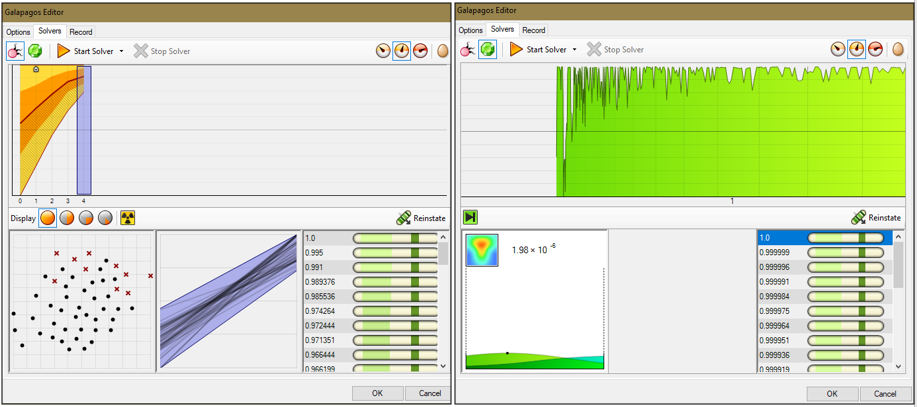
\includegraphics[width=\textwidth]{Images/Background/Galapagos/galapagos-results.PNG}
\caption[Galapagos optimization results view]{Examples of the Galapagos provided views for: (left) Genetic Algorithm, (right) Simulated Annealing algorithm}
\label{fig:galapagosvisualmenu}
\end{figure}
% End Figure -------------------------------------------------------

\subsection{Goat}
% General description, intuition
Goat is an optimization plug-in that is available in Grasshopper and exposes in a \ac{GUI} the optimization algorithms from the NLopt mathematical optimization library~\cite{NLOPT}. Simon Flöry developed Goat as a generic platform designed to use algorithms from other classes of derivative-free algorithms. Goat exposes these algorithms via an interface resemblant of Galapagos, making it easier for non-programmers to solve problems. 

% Available Algorithms
One of the key differences between Goat and Galapagos is the number and diversity of the algorithms available. Whilst Galapagos supports two global metaheuristics algorithms, Goat supports five distinct algorithms: one metaheuristic, two direct-search, and two model-based algorithms, called CRS2, DIRECT, SUBPLEX, COBYLA, and BOBYQA, respectively. Due to space constraints, a full description of these algorithms will not be provided, instead we refer the interested reader to the relevant literature.  
	
% METAHEURISTICS METHODS ------------------------------------
% CRS2
The CRS2 algorithm is a variant of the \ac{CRS} algorithm for global optimization~\cite{Price1983}. A \ac{CRS} algorithm is a population-based random search algorithm that creates an initial set of points, the population, which are then randomly evolved by means of heuristic rules. In the original \ac{CRS} algorithms, heuristic rules modify a point at a time, replacing the worst point with a better one (called trial point), using a technique resemblant of the \ac{NMS} algorithm \cite{Nelder1964}. Similarly to \ac{NMS}, \ac{CRS} algorithms use a simplex, i.e., a generalized triangle in N dimensions, to envelope a region described by a random subset of points in the population. The worst point of the population is replaced with the reflection of the worst point in the simplex~\cite{Kaelo2006CRS2}. The CRS2 variant differs from the original in that it assumes that the worst population point will always be a part of the simplex. The actual version that is made available by Goat is a modified version of the CRS2 algorithm that introduces a local mutation component in an attempt to overcome situations where heuristic rules constantly fail to find a trial points that actually improve the worst point. Fundamentally, this local mutation generates a second trial point that results from the exploitation of the region around the best point in the population~\cite{Kaelo2006CRS2}.  \todo{Vantagens e desvantagens ? Lack sound convergence properties, robustness and performance are highly problem dependent ~ler Kaelo}

% DIRECT-SEARCH METHODS ------------------------------------
% DIRECT
The second algorithm is a global deterministic direct search algorithm that relies on the division of rectangles, as explained in ~\cite{Jones1993DIRECT}. DIRECT, the DIviding RECTangles algorithm, recursively subdivides the design space into smaller multidimensional hyper-rectangles, estimating the quality value of each rectangle. DIRECT uses these values to focus the search on more promising regions of the design space and to further subdivide those in smaller hyper-rectangles. 
% SUBPLEX	
The SUBPLEX algorithm is an unconstrained local optimization algorithm~\cite{Rowan1990}. As a generalization of the \ac{NMS} algorithm, SUBPLEX subdivides the design space in low-dimensional subspaces and then applies the \ac{NMS} algorithm to a set of these subspaces, in order to seek for a better solution. In contrast to \ac{NMS}, which has difficulties in high-dimensional problems, SUBPLEX reduces the limitations through the decomposition of the problem in low-dimensional subspaces which are more efficiently optimized by \ac{NMS}.

% MODEL-BASED METHODS ------------------------------------
Besides metaheuristics and direct-search algorithms, Goat also provides two local model-based implementations, namely the COBYLA (or Constrained Optimization BY Linear Approximation) algorithm~\cite{Powell1994COBYLA}, and the BOBYQA (or Bound Optimization BY Quadratic Approximation) algorithm~\cite{Powell2009BOBYQA}, that rely on the construction of simple, partial models of the objective function~\cite{Koziel2011}. The former uses the concept of simplex to iteratively generate linear approximations of the objective function, whereas the latter generates quadratic approximations instead. 

One of the main advantages of Goat is the algorithms' diversity. By providing algorithms with different characteristics and strategies, architects can test the suitability of each algorithm to their problem and, thus, select the most effective. The right choice may result in large optimization gains, especially when complex and time-consuming simulations are necessary~\cite{Wortmann2016BBO}. For this reason, and due to the uniqueness of each \ac{BPO}, several authors suggest that the selection of the optimization algorithm should be based on the results of several tests with different algorithms for a fixed number of evaluations or a fixed amount of time~\cite{Hamdy2016,Wortmann2016BBO}. Moreover, the distinction between global and optimal algorithms is also critical when striving for accurate and precise optimal solutions. Most global optimization algorithms invest most of their effort searching for the truly optimal solution across large regions of the search space and rarely focusing on promising regions. Consequently, they might return a not so precise global optimum. To overcome this lack of precision and accuracy, one should apply a local optimization algorithm and provide the globally imprecise optimum as input.

% Usability, how to use it
%In terms of usability, Goat is very similar to Galapagos, with the only difference being the name of the input and output entries in the Goat's Grasshopper component. In Goat, the variables are connected to the entry labelled \textit{Variables}, whereas the objective function is connected to the \textit{Objective} entry. 
While in terms of usability Goat is very similar to Galapagos, it lacks the immediate feedback and post-processing features of Galapagos. On the one hand, Goat's \ac{GUI} (see \Cref{fig:goat}) is simple and easy to use for non-experts, requiring no integration efforts to use one of its optimization solvers, nor any programming or algorithm's knowledge in order to setup and use it. Moreover, the option to specify the starting point using the \textit{Sliders} components is beneficial for improving the efficiency of optimization processes.

% Begin Goat-Options Figure -------------------------------------------------------
\begin{figure}
	\centering
	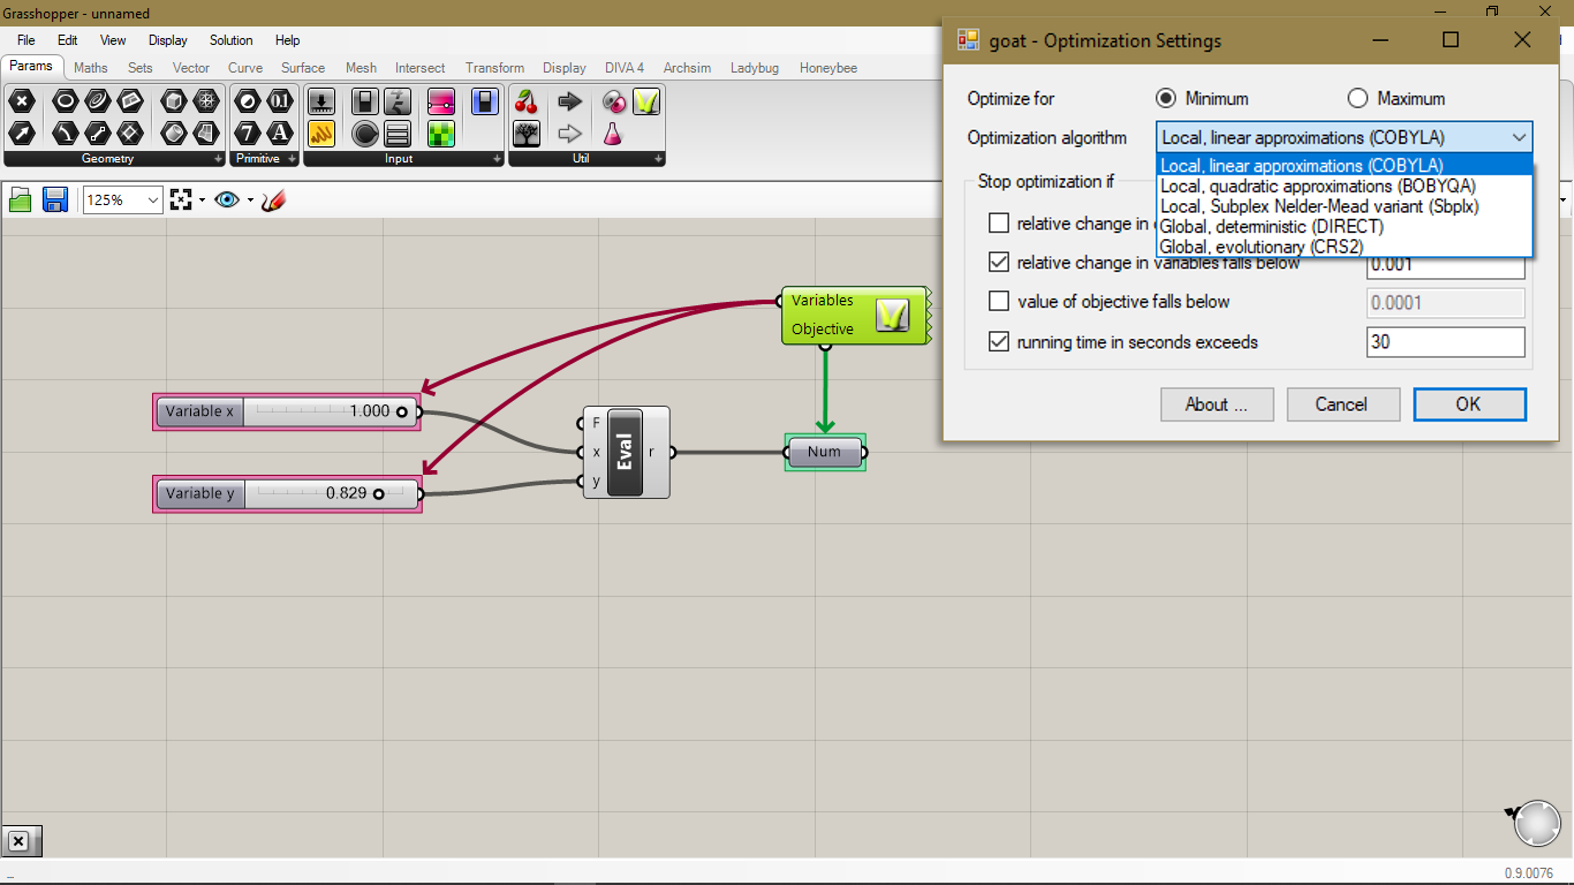
\includegraphics[width=1\textwidth]{Images/Background/Goat/general-view.png}
	\caption[Goat optimization plug-in menus]{Simple example of a Grasshopper's problem definition with two variables and a function. The Goat component is represented in green and the \textit{goat - Optimization Settings} menu lists the supported algorithms}
	\label{fig:goat}
\end{figure}
% End Figure -------------------------------------------------------	

On the other hand, Goat lacks the visual, and post-processing features. In fact, except for a final report stating the termination criteria (e.g., reach a threshold, running time exceeded), Goat provides no feedback regarding the course of the search for optimal solutions and as a result of the optimization process, Goat returns a single solution. The values for the optimal solution are exclusively exhibited using Grasshopper's \textit{Sliders}, which is not a very robust feedback mechanism (e.g., susceptible to unwilling modifications, or to information loss). In addition to bad scalability and representation of the result, Goat provides no information about other close to optimal solutions, which spurs no confidence on the achieved results.
	
\subsection{Silvereye}
Silvereye is an optimization plug-in for Grasshopper, developed under the same user interface design as Galapagos, that enables non-experts to solve complex optimization problems. Silvereye interfaces a \texttt{C\#} implementation of a single-objective \ac{PSO} algorithm.

% Algorithm
The \ac{PSO} algorithm is a global metaheuristic algorithm inspired by biological systems, such as the collective behavior of flocking birds and schooling fish, which interact and learn from one another to solve problems~\cite{Brownlee2011}. In \ac{PSO}, the intelligence is decentralized, self-organized, and distributed throughout the participating particles, also known as swarm. These particles maintain information about their velocity, their current and personal best positions, and also the global best position known to the swarm. At each time step, the position and velocity of each particle are updated according to the best swarm or close neighbor position~\cite{Brownlee2011}.

In terms of usability, Silvereye is resemblant of Galapagos, requiring the definition of Grasshopper's \textit{Sliders} as variables and a Grasshopper's \textit{Num} component as the objective function, which are then connected to the input and output entries, respectively. Upon double-clicking the Silvereye component, the user is presented with the settings menu (see \Cref{fig:silvereye}) where he is able to fine-tune the optimization solver: (1) \texttt{maximum velocity}: in each iteration, a variable can change its value by an amount that is less or equal than the value specified for this option, (2) \texttt{swarm size}: the number of particles used by the \ac{PSO} algorithm, and (3) \texttt{Use initial position}: to define one starting point, users must narrow down the range of the slider's variables, update the velocity in the solver's settings, and check this option in the Settings Menu. Moreover, Silvereye enables the user to save the solver's configurations and use them in the next run.

Silvereye supports two information mechanisms, neither of them being graphical. The first mechanism is a time log of the optimization run, discriminated by iteration and by particle. This log enables the user to control the optimization run and detect any irregularity during the run. Unfortunately, the log does not have information about the values of the solution's parameters, which makes the traceback of errors impractical. The second mechanism is a list of the best result obtained in each iteration, which can be either exported to a file or reinstantiated in Grasshopper to visualize the corresponding design. Nevertheless, similarly to the first mechanism, this list presents no explicit information about the parameters' values of explored solutions and the user is restricted to the best result listed, not being able to verify other close to optimal solutions that might have been explored in the course of the optimization.

% Begin Silvereye-Options Figure -------------------------------------------------------
\begin{figure}
	\centering
	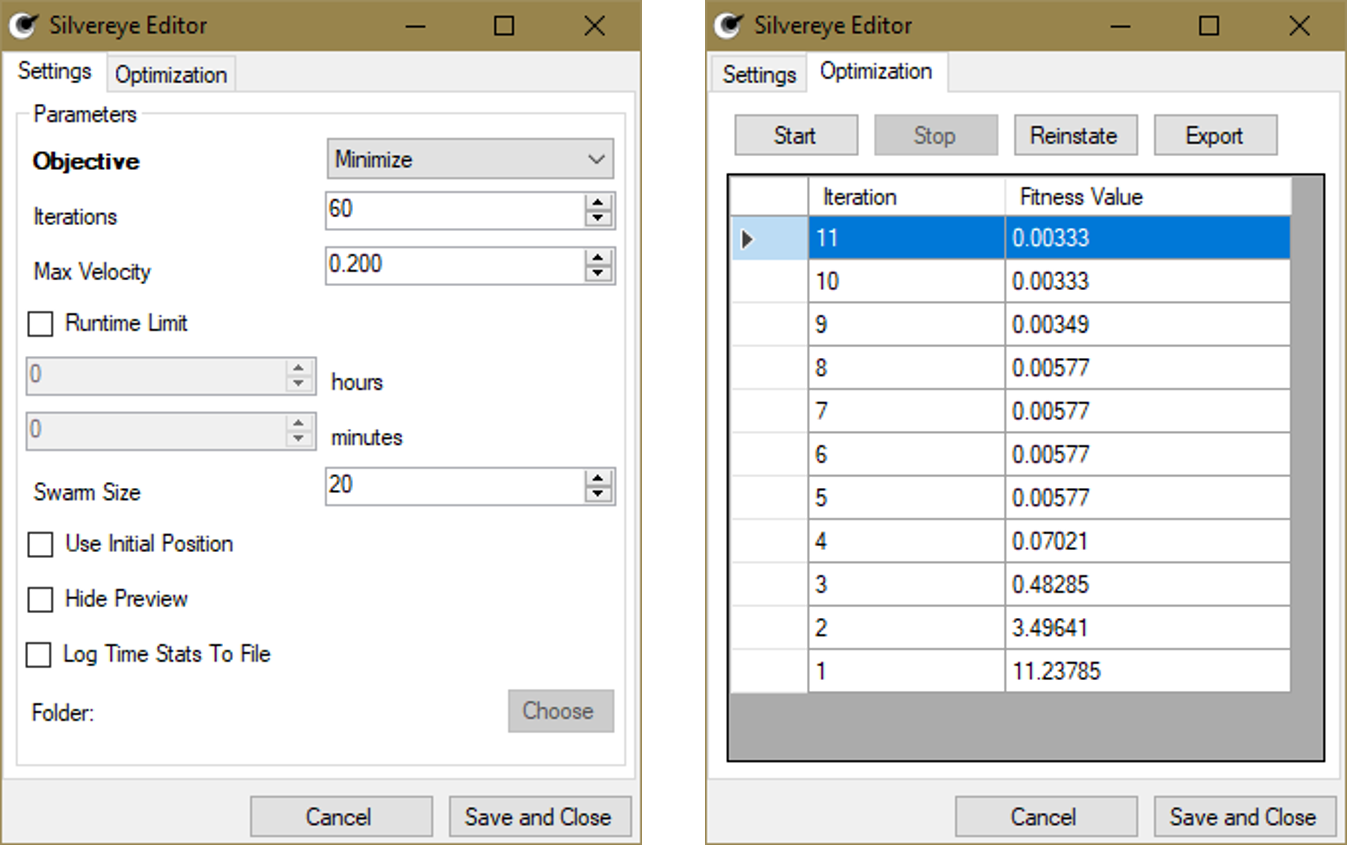
\includegraphics[width=0.5\textwidth]{Images/Background/Silvereye/general-view.png}
	\caption[Silvereye optimization plug-in menus]{The Silvereye Editor menus: (left) Settings menu, (right) Optimization results}
	\label{fig:silvereye}
\end{figure}
% End Figure -------------------------------------------------------	

\subsection{Opossum}

Opossum (OPtimizatiOn Systems with SUrrogate Models) is a single-objective plug-in developed for Grasshopper that interfaces the model-based RBFOpt library~\cite{RBFOPT}. Its \ac{GUI} is similar to the one of Galapagos.

Opossum is a model-based optimization tool for Grasshopper that uses the \ac{RBF} machine learning technique to create global approximations of the objective function~\cite{Forrester2009SBO}. These approximations are simply the weighted sum of other, simpler, real-valued functions, the radial functions. These functions are defined on the Euclidean space $\mathbb{R}^n$ and their value depends on the distance to a center $c$, so that $\phi(x, c) = \phi(\left\lVert x-c \right\rVert)$. In a \acp{RBF} technique, the weights are estimated based on the interpolation of data. A comprehensive detailed explanation of the \ac{RBF}'s estimation process is provided in~\cite{Forrester2009SBO}. 

Since its invention, multiple implementations of \ac{RBF} have been proposed. RBFOpt implements two well-known versions, namely, the Gutmann's~\cite{Gutmann2001} and the Regis and Shoemaker's~\cite{Regis2007}, commonly known as MSRSM. These techniques differ in the search strategy for the next candidate solution to be evaluated using the original objective function. The former uses the solution, which is likely to yield the largest improvement in the surrogate's accuracy, whereas the latter tries to balance the surrogate's accuracy amelioration with the exploitation of promising solutions, using other search strategies, such as genetic algorithms, sampling algorithms, or other mathematical solvers~\cite{Wortmann2017Opossum}. Moreover, RBFOpt provides five different types of radial basis function: linear, multi-quadratic, cubic, thin plate spline, and automatic selection, which are also provided in the Opossum interface.

In terms of usability, Opossum resembles Galapagos. In contrast to other plug-ins, Opossum provides a more flexible interface, with menus tailored for different expertise levels, offering different levels of control in each one. By providing multiple menus (see~\Cref{fig:opossum}), both less and more experienced users are able to use a tool that suits their needs, while providing the more experienced ones the ability to fine-tune the optimization solvers more accurately, thus potentially achieving more efficient optimization processes.

One other important aspect of Opossum is concerned with the exposition of results. On the one hand, Opossum provides a graphical view of the best value ever found up to each iteration (see~\Cref{fig:opossum}-left), thus providing immediate feedback to the architect about the state of the optimization process. On the other hand, Opossum can create a log file with the record of all the solutions explored during the optimization process. This log file can then be used with other post-processing tools for purposes of more insightful visualizations of the data, or even to re-use this information to perform sensitivity analysis or to run other optimization algorithms (e.g., benchmarks).

% Begin Opossum-Options Figure -------------------------------------------------------
\begin{figure}
	\centering
	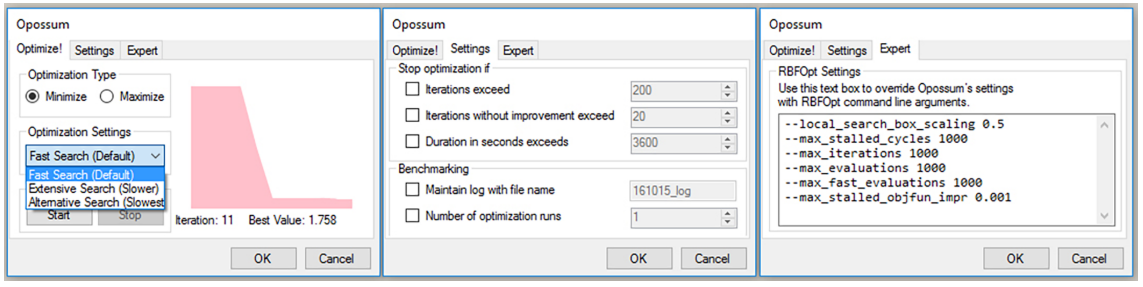
\includegraphics[width=1\textwidth]{Images/Background/Opossum/opossum_1.png}
	\caption[Opossum optimization plug-in menus]{The three menus of the Opossum's \ac{GUI}}
	\label{fig:opossum}
\end{figure}
% End Figure -------------------------------------------------------

\subsection{Octopus}

Octopus is a multi-objective plug-in developed for Grasshopper. Designed in the same way as Galapagos, Octopus exploits evolutionary principles to search for multiple Pareto-optimal solutions.  

The installation of Octopus creates a new tab within Grasshopper, which encloses seven menus discriminated by different functionality, including Evolutionary Learning, Octopus, Supervised Learning, among others. Octopus enables the simultaneous search for more than one objective, producing a set of possible optimal solutions that ideally represent the real trade-offs between each objective. In order to search for the Pareto-optimal solutions, Octopus provides two main evolutionary algorithms: \ac{SPEA2} and \ac{HypE}. On the one hand, due to their population-based nature, evolutionary algorithms are able to approximate the Pareto Front in a single run~\cite{Zhou2011}. On the other hand, these algorithms have been reported to yield promising results on numerous test problems~\cite{Zitzler2001SPEA2,Zitzler2011HypE}.

Similarly to evolutionary algorithms, \acp{MOEA} adopt the evolutionary principles discussed in \cref{subsec:galapagos} but, generally, have an additional archive to store the non-dominated solutions found~\cite{Zitzler2001SPEA2}. The archive technique is incorporated to prevent losing current non-dominated solutions due to random mutations or recombinations. Most \acp{MOEA} differ in the selection and reproduction operators used to iteratively evolve populations. These differences are usually related to the very own goals of approximating the Pareto Front: (1) maximize the accuracy of the approximation (by minimizing the distance to the optimal front) and (2) maximize the diversity of the solutions within the front. While the first goal is related to the search strategy and how to assign fitness values in such a way that the individuals selected for offspring production will be closer to the Pareto-optimal front, the second goal is related to the time and storage constrains of the evolution process and which individuals to keep in each generation \cite{Zitzler2001SPEA2}. Although a thorough description of different \acp{MOEA} and their mechanisms is not herein presented, we refer the interested reader to \cite{Zhou2011}. 
	
Most modern \acp{MOEA} realize the accuracy and diversity ideas through some implementation of the following mechanisms~\cite{Zitzler2001SPEA2}:	
\begin{itemize}
\item Selection (or environmental selection): Besides the population, most \acp{MOEA} maintain an archive with the non-dominated front among all the solutions that were evaluated. The archive preserves individuals during several generations, only removing them if (1) a new solution is found to dominate them, or (2) if the archive size is exceeded and they happen to be in crowded regions of the front.

\item Reproduction (or mating selection): At each generation, individuals are evaluated in two stages. The first stage compares them regarding the relation of Pareto dominance, using this information to define a ranking among these individuals. The second stage refines these rankings through the incorporation of density information, i.e., if the individuals lie in crowded regions.
\end{itemize}

These mechanisms can be completely indifferent from one another, e.g., the first one applying a Pareto-based criteria and the second one applying weighting approach. However, many \acp{MOEA} implement both concepts similarly. In the particular case of \ac{SPEA2}, the algorithm explores two independent sets of individuals: the population and the archive. In this algorithm, the archive size is fixed and, therefore, whenever the number of non-dominated individuals is less than its size, some dominated individuals are added to the archive. At each iteration, the algorithm computes each individual's fitness value (a \textit{strength} value, defined as terms of the number of solutions it dominates, the \textit{raw fitness} value, defined in terms of the strength of its dominators, and a density estimate, defined as the inverse of the distance to the $k^{th}$ to the nearest neighbor) and copies the non-dominated individuals from the population to the archive, removing any individual that is dominated, whose objective values are duplicated, or that, when the size of the updated archive is exceeded, lies in crowded regions of the non-dominated front. After filling the archive, pairs of individuals are chosen from the archive to reproduce and produce the offspring through recombination and mutation operators that will make the population of the next generation~\cite{Zitzler2001SPEA2}.
	
Unfortunately, algorithms incorporating the Pareto dominance relation and diversity measures appear to have difficulties in optimization scenarios with more than two objectives, which spurred the development of algorithms using other quality measures, including quality indicators. To overcome the objective limitation and provide the user with the flexibility to use a more efficient algorithm, Octopus provides the option to use \ac{HypE}, an algorithm that explores the \ac{HV} indicator to rank individuals. Particularly, to minimize time penalties associated with the computation of the \ac{HV}, in scenarios with more than three objectives, \ac{HypE} uses Monte Carlo simulations to estimate the \ac{HV} value of each individual~\cite{Zitzler2011HypE}. 

% 	https://pdfs.semanticscholar.org/dbc6/99826d7d28a75a304e715b796c8d2ee3dc90.pdf
	
% Begin Octopus-Options Figure -------------------------------------------------------
\begin{figure}
\centering
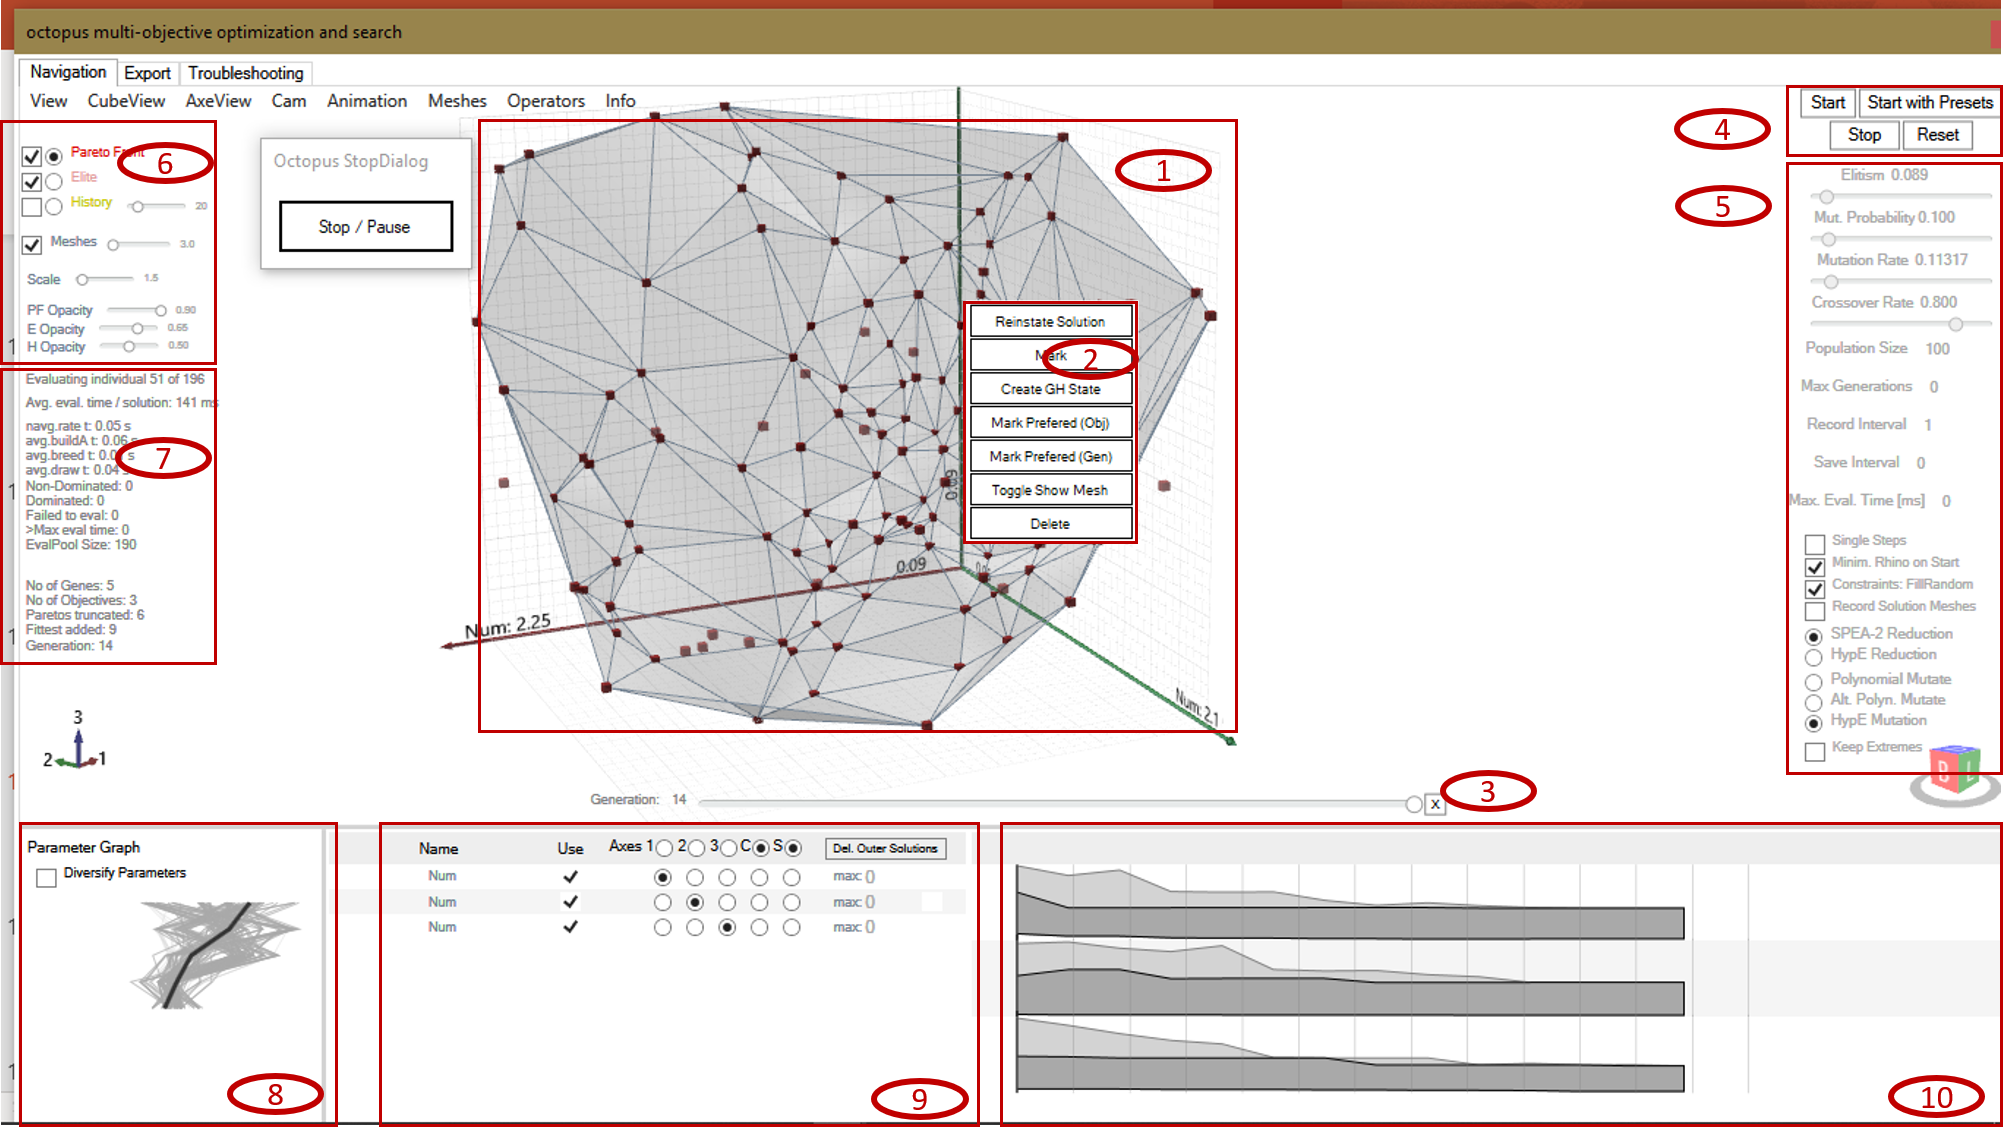
\includegraphics[width=1\textwidth]{Images/Background/Octopus/octopus-menu.png}
\caption[Octopus optimization plug-in Editor]{Octopus Editor: (1) Solutions' Objective Space, (2) Solution's context menu, (3) Generation's history slider, (4) Process control options, (5) Algorithm Settings, (6) Display Settings, (7) Statistics, (8) Parallel Coordinates Graph, (9) List of Objectives (10) Convergence graphs per Objective}
\label{fig:octopus}
\end{figure}
% End Figure -------------------------------------------------------	

% Usability
% there is not a clear separation of different menus and their position in the menu seems to be counter intuitive (e.g., algorithm and process control options on the right, and display options on the left). 
In terms of usability, Octopus is very similar to Galapagos. \Cref{fig:octopus} illustrates the Octopus editor after running \ac{SPEA2} for fourteen generations for a 3-objective optimization problem. This interface lacks organization of its functionalities and is overloaded with information, thus hindering its overall usability and comprehension.

One key aspect of this interface is the ability to configure multiple parameters of both the algorithm and the optimization run, even during runtime. Moreover, by default, Octopus disables the real-time design generation of design candidates with the aim of reducing time penalizations. The consequence of such option is an optimization process where no information is provided to the user.

Another key aspect of this interface is the post-processing and visualization mechanisms. On the one hand, it provides multiple views of the evolution of the optimization process (see views 1, 8, and 10 in \Cref{fig:octopus}). While these views provide a comprehensive feedback about the course of optimization for problems with less than or equal to five objectives (e.g., using color and dimension as additional features), it is unclear how Octopus represents solutions with more than five objectives in the main view port. On the other hand, it allows the user to export different information to files. 

\subsection{Optimo}
\label{subsec:Optimo}

Implemented on top of Dynamo, Optimo is an evolutionary-based multi-objective optimization plugin that enables users to optimize both single and multi-objective problems. The current version of Optimo uses an \ac{NSGA-II} \cite{Deb2002} from the jMetal.NET library to seek for Pareto-Optimal solutions. 

% Algoritmo
As a \ac{MOEA}, \ac{NSGA-II} attempts to achieve an approximation to the Pareto front that is both accurate and diverse. In this particular algorithm, both the selection and reproduction mechanisms rely on the same basis criteria: Pareto dominance relations and a crowding measure. To define the order among the individuals, the pool of individuals is split into different Pareto fronts and ranked accordingly, i.e., the first non-dominated front is assigned the highest rank, the second front is assigned the second highest rank, and so on. Each individual in each rank is ordered according to a crowding measure, represented in terms of the sum of distances to the two closest individuals along each objective. The archive and the generation's population are combined, deleting the worst 50\%. Afterwards, binary tournaments are carried out on the remaining individuals (the archive members) in order to generate the next offspring population.

% USABILIDADE (ligações caixinhas, parametros)
In order to help designers optimize multiple conflicting objectives and approach to a set of optimal solutions, Optimo includes four nodes in Dynamo: (1) Initial Solution List, which generates the initial set of random design configurations within a provided range and with the specified size of population; (2) Assign Fitness Function Results, which evaluates and assigns the objective values to each configuration; (3) Generation Algorithm, which takes the parent population and generates the children population; and (4) Sorting, which uses the Pareto Front sorting to sort the solutions. Comparing to the other plug-ins, Optimo presents more detailed and complex node structure, as it provides the user four different blocks to manipulated instead of enclosing them in a single abstraction.

% Visual
Regarding the post-processing features, Optimo creates a CSV file with the results of the optimization run. However, it provides no visual feedback about the evolution of the optimization run nor about the best evaluated solutions, thus lacking post-processing features and requiring the usage of external applications or frameworks.

% Comparison
\subsection{Comparison}




% #############################################################################
\section{Problems to Address}

